\documentclass[10pt, a5paper]{article}
\usepackage{pdfpages}
\usepackage{parallel}
\usepackage[T2A]{fontenc}
\usepackage{ucs}
\usepackage[utf8x]{inputenc}
\usepackage[polish,english,russian]{babel}
\usepackage{hyperref}
\usepackage{rotating}
\usepackage[inner=2cm,top=1.8cm,outer=2cm,bottom=2.3cm,nohead]{geometry}
\usepackage{listings}
\usepackage{graphicx}
\usepackage{wrapfig}
\usepackage{longtable}
\usepackage{indentfirst}
\usepackage{array}
\newcolumntype{P}[1]{>{\raggedright\arraybackslash}p{#1}}
\frenchspacing
\usepackage{fixltx2e} %text sub- and superscripts
\usepackage{icomma} % коскі ў матэматычным рэжыме
\PreloadUnicodePage{4}

\newcommand{\longpage}{\enlargethispage{\baselineskip}}
\newcommand{\shortpage}{\enlargethispage{-\baselineskip}}

\def\switchlang#1{\expandafter\csname switchlang#1\endcsname}
\def\switchlangbe{
\let\saverefname=\refname%
\def\refname{Літаратура}%
\def\figurename{Іл.}%
}
\def\switchlangen{
\let\saverefname=\refname%
\def\refname{References}%
\def\figurename{Fig.}%
}
\def\switchlangru{
\let\saverefname=\refname%
\let\savefigurename=\figurename%
\def\refname{Литература}%
\def\figurename{Рис.}%
}

\hyphenation{admi-ni-stra-tive}
\hyphenation{ex-pe-ri-ence}
\hyphenation{fle-xi-bi-li-ty}
\hyphenation{Py-thon}
\hyphenation{ma-the-ma-ti-cal}
\hyphenation{re-ported}
\hyphenation{imp-le-menta-tions}
\hyphenation{pro-vides}
\hyphenation{en-gi-neering}
\hyphenation{com-pa-ti-bi-li-ty}
\hyphenation{im-pos-sible}
\hyphenation{desk-top}
\hyphenation{elec-tro-nic}
\hyphenation{com-pa-ny}
\hyphenation{de-ve-lop-ment}
\hyphenation{de-ve-loping}
\hyphenation{de-ve-lop}
\hyphenation{da-ta-ba-se}
\hyphenation{plat-forms}
\hyphenation{or-ga-ni-za-tion}
\hyphenation{pro-gramming}
\hyphenation{in-stru-ments}
\hyphenation{Li-nux}
\hyphenation{sour-ce}
\hyphenation{en-vi-ron-ment}
\hyphenation{Te-le-pathy}
\hyphenation{Li-nux-ov-ka}
\hyphenation{Open-BSD}
\hyphenation{Free-BSD}
\hyphenation{men-ti-on-ed}
\hyphenation{app-li-ca-tion}

\def\progref!#1!{\texttt{#1}}
\renewcommand{\arraystretch}{2} %Іначай формулы ў матрыцы зліпаюцца з лініямі
\usepackage{array}

\def\interview #1 (#2), #3, #4, #5\par{

\section[#1, #3, #4]{#1 -- #3, #4}
\def\qname{LVEE}
\def\aname{#1}
\def\q ##1\par{{\noindent \bf \qname: ##1 }\par}
\def\a{{\noindent \bf \aname: } \def\qname{L}\def\aname{#2}}
}

\def\interview* #1 (#2), #3, #4, #5\par{

\section*{#1\\{\small\rm #3, #4. #5}}

\def\qname{LVEE}
\def\aname{#1}
\def\q ##1\par{{\noindent \bf \qname: ##1 }\par}
\def\a{{\noindent \bf \aname: } \def\qname{L}\def\aname{#2}}
}


\begin{document}

\title{Применение свободного ПО при создании и внедрении Системы контроля за выполнением поручений Правительства}% данных и последующих тезисов, кроме специально оговоренных случаев, доступен под лицензией Creative Commons Attribution-ShareAlike 3.0}

\author{Максим Радюк\footnote{Минск, Belarus}}
\maketitle

\begin{abstract}
One of the main functions of the Council of Ministers of the Republic of Belarus is to control the realization of the government orders. To improve the organizational and technical issues of the order control in the automated information system of the Council of Ministers, the automated System of Control presented here was recently developed.
This system is based on free / open source software and therefore does not require additional investment. Being a part of the electronic documents circulation of the Council of Ministers the System of Control is accessible through the infrastructures of both the Council of Ministers and e-mail (mailgov.by) of other executives. The core of the System uses Ubuntu Server with HTTP and XMPP protocols. Its client part requires Sencha Ext JS in the browser of and allows review of orders to execute, including information about the process, and final report in the executive affiliation.
Currently the System of Control is in active development being exploited in 67 executives in the Republic of Belarus.
\end{abstract}

\textbf{Описание и цели создания}

Одной из основных функций Аппарата Совета Министров Республики Беларусь (Аппарат) является контроль за выполнением органами государственного управления поручений, поступающих от Премьер-министра, заместителей Премьер-министра Республики Беларусь.  До недавнего времени существующий технический порядок обработки поручений в аппаратно-программной платформе подсистем делопроизводства и контроля исполнения поручений (АПП) автоматизированной системы обработки информации \linebreak (АСОИ) Аппарата учитывал не все организационные и технические моменты контроля поручений Правительства, что затрудняло оперативное решение поставленных задач.

Информацию о постановке на контроль и напоминания о приближении сроков исполнения поручений органы государственного управления получали по электронной почте. Ответственному работнику Аппарата приходилось по телефону выяснять, кто является непосредственным исполнителем поручения в органе государственного управления. Также, на стороне госоргана, отсутствовала возможность внесения информации об исполнении того или иного поручения.

Для совершенствования существующей инфраструктуры в инициативном порядке было принято решение о создании Системы контроля за выполнением поручений Правительства (Система контроля).

Система контроля обеспечивает организацию единого информационного процесса  контроля за выполнением поручений Правительства независимо от внутриведомственной деятельности пользователей и  выполняет следующие функции:

\begin{itemize}
  \item просмотр списка активных и исполненных поручений
  \item печать списка поручений
  \item получение информации об исполнителе поручения в госоргане
  \item получение информации о выполнении поручения в госоргане
  \item получение информации о соисполнителях поручения в других госорганах
  \item поиск поручений по реквизитам
  \item формирование справочников
  \item отправка почтовых сообщений работникам Аппарата
  \item обмен мгновенными сообщениями между работниками Аппарата и работниками других госорганов (в разработке).
\end{itemize}

\textbf{Архитектура}

Схема на рис. \ref{R1} представляет положение Системы контроля в структуре АСОИ Аппарата.

\begin{figure}[htpb]
  \centering
  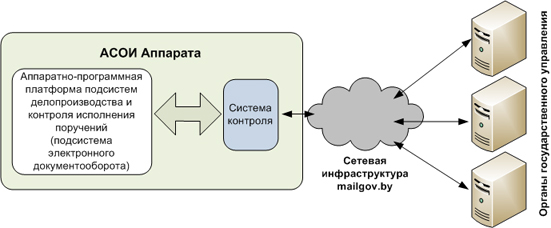
\includegraphics[width=9cm]{110_2012_w_cmcntrlsys_figure1_1.jpg}
\caption{Система контроля внутри АСОИ Аппарата}
\label{R1}
\end{figure}

Система контроля является надстройкой над подсистемой электронного документооборота АСОИ Аппарата и представляет собой веб-ресурс , доступный как из инфраструктуры АСОИ Аппарата, так и через сетевую инфраструктуру электронной почты государственных органов mailgov.by.

Структурная схема Системы контроля изображена на рис. \ref{R2} и состоит из следующих компонент:

\begin{itemize}
  \item основной сервер, доступный по адресу \url{http://cmcntlsys.cm.by}
  \item реплика-сервер
  \item ftp-сервер обмена данными
  \item корпоративный контроллер домена Active Directory
  \item xmpp (jabber) --- сервер обмена мгновенными сообщениями.
\end{itemize}

\begin{figure}[htpb]
  \centering
  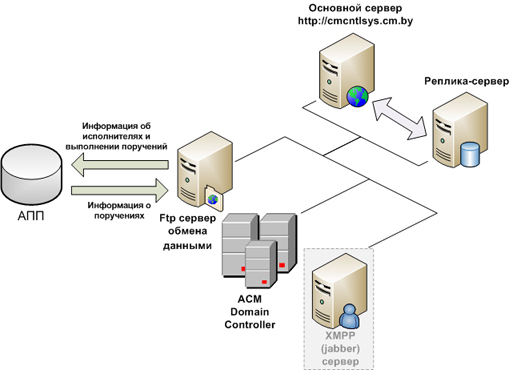
\includegraphics[width=9cm]{110_2012_w_cmcntrlsys_figure2_1.jpg}
\caption{Структурная схема Системы контроля}
  \label{R2}
\end{figure}
Серверная часть (ядро) аккумулирует всю информацию о ходе процесса контроля выполнения поручений и обеспечивает предоставление информации пользователям.  Обмен данными между Системой контроля и АПП Аппарата обеспечивается по ftp-протоколу через выделенный сервер. Ядро Системы контроля построено с использованием следующих продуктов и технологий:

\begin{itemize}
  \item операционная система: Ubuntu Server 10.10
  \item web-сервер: Apache 2.2.16
  \item СУБД: MySQL 5.1.49
  \item язык разработки: PHP 5.3.3
  \item XMPP-сервер: Openfire 3.7.1.
\end{itemize}

Клиентская часть Системы контроля представляет собой приложение, разработанное с использованием javascript-библиотек Sencha Ext JS 3.3.0., выполняемое в браузере пользователя. Основное её предназначение --- просмотр списка поручений, подлежащих исполнению, а также внесение информации и отчета об исполнении поручения в органе государственного управления.

Выбор свободного программного обеспечения при разработке Системы контроля обусловлен следующими факторами:

\begin{itemize}
  \item отсутствуют какие-либо дополнительные финансовые затраты;
  \item нет необходимости осуществления обязательных процедур \linebreak обоснования, согласования и проведения тендеров на закупку ПО --- т.н. <<быстрый старт>>.
\end{itemize}

В настоящее время ведется активное развитие и опытная эксплуатация Системы контроля в 67 органах государственного управления. В презентации мы представим более подробную информацию о порядке работы в Системе контроля, пользовательский интерфейс и разъясним технические детали реализации проекта.



\end{document}




